\documentclass[a4paper, 12pt,twoside]{book}\usepackage[]{graphicx}\usepackage[]{color}
%% maxwidth is the original width if it is less than linewidth
%% otherwise use linewidth (to make sure the graphics do not exceed the margin)
\makeatletter
\def\maxwidth{ %
  \ifdim\Gin@nat@width>\linewidth
    \linewidth
  \else
    \Gin@nat@width
  \fi
}
\makeatother

\definecolor{fgcolor}{rgb}{0.345, 0.345, 0.345}
\newcommand{\hlnum}[1]{\textcolor[rgb]{0.686,0.059,0.569}{#1}}%
\newcommand{\hlstr}[1]{\textcolor[rgb]{0.192,0.494,0.8}{#1}}%
\newcommand{\hlcom}[1]{\textcolor[rgb]{0.678,0.584,0.686}{\textit{#1}}}%
\newcommand{\hlopt}[1]{\textcolor[rgb]{0,0,0}{#1}}%
\newcommand{\hlstd}[1]{\textcolor[rgb]{0.345,0.345,0.345}{#1}}%
\newcommand{\hlkwa}[1]{\textcolor[rgb]{0.161,0.373,0.58}{\textbf{#1}}}%
\newcommand{\hlkwb}[1]{\textcolor[rgb]{0.69,0.353,0.396}{#1}}%
\newcommand{\hlkwc}[1]{\textcolor[rgb]{0.333,0.667,0.333}{#1}}%
\newcommand{\hlkwd}[1]{\textcolor[rgb]{0.737,0.353,0.396}{\textbf{#1}}}%
\let\hlipl\hlkwb

\usepackage{framed}
\makeatletter
\newenvironment{kframe}{%
 \def\at@end@of@kframe{}%
 \ifinner\ifhmode%
  \def\at@end@of@kframe{\end{minipage}}%
  \begin{minipage}{\columnwidth}%
 \fi\fi%
 \def\FrameCommand##1{\hskip\@totalleftmargin \hskip-\fboxsep
 \colorbox{shadecolor}{##1}\hskip-\fboxsep
     % There is no \\@totalrightmargin, so:
     \hskip-\linewidth \hskip-\@totalleftmargin \hskip\columnwidth}%
 \MakeFramed {\advance\hsize-\width
   \@totalleftmargin\z@ \linewidth\hsize
   \@setminipage}}%
 {\par\unskip\endMakeFramed%
 \at@end@of@kframe}
\makeatother

\definecolor{shadecolor}{rgb}{.97, .97, .97}
\definecolor{messagecolor}{rgb}{0, 0, 0}
\definecolor{warningcolor}{rgb}{1, 0, 1}
\definecolor{errorcolor}{rgb}{1, 0, 0}
\newenvironment{knitrout}{}{} % an empty environment to be redefined in TeX

\usepackage{alltt}

% set the paper size and the margins
\usepackage[top = 2cm, bottom = 2cm, left = 2cm, right = 3cm ]{geometry}
% set the header and the footnote
\usepackage{fancyhdr}
\pagestyle{fancy}
\fancyhf{}
\fancyhead[CE,CO]{Exploratory Analysis}
\fancyfoot[LE,RO]{\thepage}
% Supress the hyphenation
\hyphenation{thatshouldnot}
% define a color for highlight
\definecolor{asparagus}{rgb}{0.53, 0.66, 0.42}
\definecolor{babypink}{rgb}{0.96, 0.76, 0.76}
\definecolor{champagne}{rgb}{0.97, 0.91, 0.81}
\definecolor{forestgreen}{rgb}{0.13, 0.55, 0.13}
\definecolor{dollarbill}{rgb}{0.52, 0.73, 0.4}

% packages will be used by the 'kable' package
\usepackage{booktabs}
\usepackage{longtable}
\usepackage{array}
\usepackage{multirow}
\usepackage[table]{xcolor}
\usepackage{wrapfig}
\usepackage{float}
\usepackage{colortbl} 
\usepackage{pdflscape}
\usepackage{tabu}
\usepackage{threeparttable}
\usepackage{threeparttablex}
\usepackage[normalem]{ulem}
\usepackage{makecell}
\usepackage{xcolor}

% For somes graphs imported from outside sources
\usepackage{graphicx}
\IfFileExists{upquote.sty}{\usepackage{upquote}}{}
\begin{document}

\chapter{Exploratory Analysis}
\thispagestyle{empty}
Statistics is a science of data. To study statistics, we have to describe data from some proper perspectives. Generally speaking, there are two ways to describe data, graphical description and numerical description. Those are what we are going to learn in this section.
\newpage

\section{Basic concepts}
\begin{center}
\begin{knitrout}
\definecolor{shadecolor}{rgb}{0.969, 0.969, 0.969}\color{fgcolor}\rowcolors{2}{gray!6}{white}
\begin{table}[!h]

\caption{\label{tab:unnamed-chunk-1}Final scores}
\centering
\begin{tabular}[t]{ccccc}
\hiderowcolors
\toprule
Names & Student.id & Calculus & Physics & Gender\\
\midrule
\showrowcolors
James & 170101 & 75 & 74 & Male\\
Sam & 170102 & 87 & 83 & Male\\
Crystal & 170103 & 88 & 92 & Female\\
Evelyne & 170104 & 84 & 82 & Female\\
Phoebe & 170105 & 89 & 86 & Female\\
\addlinespace
Vince & 170106 & 76 & 85 & Male\\
Mike & 170107 & 71 & 76 & Male\\
Allen & 170108 & 73 & 60 & Male\\
Lucy & 170109 & 81 & 89 & Female\\
Kitty & 170110 & 86 & 91 & Female\\
\addlinespace
Owen & 170111 & 88 & 82 & Male\\
Angela & 170112 & 96 & 93 & Female\\
Christina & 170113 & 87 & 81 & Female\\
Jamie & 170114 & 84 & 80 & Female\\
Meggie & 170115 & 80 & 82 & Female\\
\addlinespace
Kevin & 170116 & 97 & 99 & Male\\
Tom & 170117 & 90 & 86 & Male\\
Lunna & 170118 & 85 & 62 & Female\\
John & 170119 & 81 & 88 & Male\\
Jason & 170120 & 72 & 80 & Male\\
\bottomrule
\end{tabular}
\end{table}
\rowcolors{2}{white}{white}


\end{knitrout}
\end{center}
\begin{itemize}
\item \textit{Table 1.1} gives the final scores of 20 students, each student is an \textbf{individual}. 
\item All stduents are described through  \textit{Names, Students id, Calculus, Physics}, and \textbf{Gender}. They are called \textbf{Variables}, for they may take different values for different individual.s

\item The values of \textit{Calculus} and \textit{Physics} can be manipulated as usual numbers. \textit{Calculus} and \textit{Physics} are called \textbf{quantitative variables}.

\item The values of \textit{Names, Students id} and \textit{Gender} can not be manipulated as usual numbers. They are called \textbf{categorical variables}.

\item The way a variable takes different values is call the \textbf{distribution} of this variable.

\end{itemize}

\section{Graphical displays}
\begin{itemize}

\item \textbf{Bar Graph}, a graph to show the distribution of \colorbox{babypink}{categorical variables}.

\begin{knitrout}
\definecolor{shadecolor}{rgb}{0.969, 0.969, 0.969}\color{fgcolor}\begin{figure}[H]

{\centering \includegraphics[width=\maxwidth]{figure/unnamed-chunk-2-1} 

}

\caption[\label{barplot} Bar graph for the distribution of the Gender]{\label{barplot} Bar graph for the distribution of the Gender}\label{fig:unnamed-chunk-2}
\end{figure}


\end{knitrout}
\colorbox{babypink}{Be sure to indicate the labels of the aixes whenever a graph is drawn}\\

The vertical axis of \textit{figure} \ref{barplot}  is \textbf{frequency}, which means the number of individuals. \textit{Figure} \ref{barplot} means there are 10 male students and 10 female students. 

Sometimes the vertical axis can be \textbf{relative frequency}, as shown in \textit{figure}\ref{barplot_relative}. It means $50\%$ of the students are male and $50\%$ are female.
\begin{knitrout}
\definecolor{shadecolor}{rgb}{0.969, 0.969, 0.969}\color{fgcolor}\begin{figure}[H]

{\centering \includegraphics[width=\maxwidth]{figure/unnamed-chunk-3-1} 

}

\caption[\label{barplot_relative} Bar graph for the distribution of the Gender]{\label{barplot_relative} Bar graph for the distribution of the Gender}\label{fig:unnamed-chunk-3}
\end{figure}


\end{knitrout}
\item \textbf{Dot plot}
\begin{knitrout}
\definecolor{shadecolor}{rgb}{0.969, 0.969, 0.969}\color{fgcolor}\begin{figure}[H]

{\centering \includegraphics[width=\maxwidth]{figure/unnamed-chunk-4-1} 

}

\caption[\label{dotplot_cal} Dot plot for the distribution of the Calculus scores]{\label{dotplot_cal} Dot plot for the distribution of the Calculus scores}\label{fig:unnamed-chunk-4}
\end{figure}


\end{knitrout}

\item \textbf{Histogram}
\begin{knitrout}
\definecolor{shadecolor}{rgb}{0.969, 0.969, 0.969}\color{fgcolor}\begin{figure}[H]

{\centering \includegraphics[width=\maxwidth]{figure/unnamed-chunk-5-1} 

}

\caption[\label{histogram_cal} Histogram for the distribution of the Calculus scores]{\label{histogram_cal} Histogram for the distribution of the Calculus scores}\label{fig:unnamed-chunk-5}
\end{figure}


\end{knitrout}
\colorbox{dollarbill}{What is the difference between the bar graph and histogram?}

\item \textbf{Stemplots}
\begin{figure}[!ht]
\centering
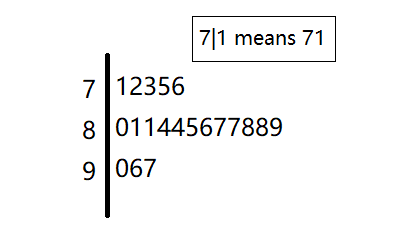
\includegraphics[scale=1]{figure1.png}
\caption{Stem plot for the distribution of calculus scores}
\label{stemplot_cal}
\end{figure}

\colorbox{babypink}{Don't forget the legend}\\
\end{itemize}

\end{document}

